\documentclass[tikz,border=2mm]{standalone} 
\usetikzlibrary{positioning, shapes}

\begin{document}
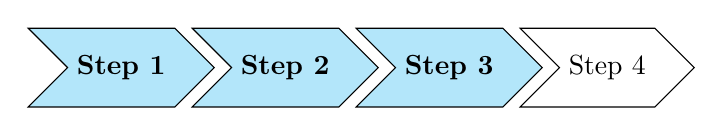
\begin{tikzpicture}[
    myarrow/.style={signal, signal from=west, draw, fill=#1, minimum height=1cm, minimum width=2cm},
    node distance=2mm]

\node[myarrow=cyan!30](a){\textbf{Step 1}};
\node[myarrow=cyan!30, right=of a](b){\textbf{Step 2}};
\node[myarrow=cyan!30, right=of b](c){\textbf{Step 3}};
\node[myarrow=cyan!0, right=of c](d){Step 4};
\end{tikzpicture}


\end{document}